\section{Εισαγωγή}

\section{Τι είναι ο κατακερματισμός;}
Ο κατακερματισμός (hashing) είναι μια μέθοδος που επιτυγχάνει ταχύτατη αποθήκευση και αναζήτηση δεδομένων. Σε ένα σύστημα κατακερματισμού τα δεδομένα αποθηκεύονται σε έναν πίνακα που ονομάζεται πίνακας κατακερματισμού (hash table). Εφαρμόζοντας στο κλειδί κάθε εγγραφής που πρόκειται να αποθηκευτεί ή να αναζητηθεί τη συνάρτηση κατακερματισμού (hash function) προσδιορίζεται μονοσήμαντα η θέση του πίνακα στην οποία τοποθετούνται τα δεδομένα της εγγραφής.
Μια καλή συνάρτηση κατακερματισμού θα πρέπει να κατανέμει τα κλειδιά στα κελιά του πίνακα κατακερματισμού όσο πιο ομοιόμορφα γίνεται και να είναι εύκολο να υπολογιστεί.

\begin{figure}[h]
\centering
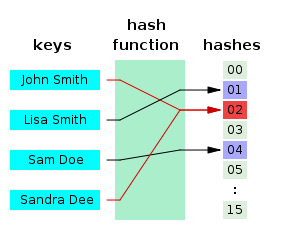
\includegraphics{HashTable.png}
\caption{}
\label{fig:hashtable1}
\end{figure}

Είναι επιθυμητό το παραγόμενο αποτέλεσμα από τη συνάρτηση κατακερματισμού να εξαρτάται από το κλειδί στο σύνολό του.

Οι πίνακες κατακερματισμού είναι ιδιαίτερα κατάλληλοι για εφαρμογές στις οποίες πραγματοποιούνται συχνές αναζητήσεις εγγραφών με δεδομένες τιμές κλειδιών. Ωστόσο, οι πίνακες κατακερματισμού έχουν και μειονεκτήματα καθώς είναι δύσκολο να επεκταθούν από τη στιγμή που έχουν δημιουργηθεί και μετά. Επίσης, η απόδοσή των πινάκων κατακερματισμού υποβαθμίζεται καθώς οι θέσεις τους γεμίζουν με στοιχεία. Συνεπώς, εφόσον ο προγραμματιστής προχωρήσει στη δική του υλοποίηση ενός πίνακα κατακερματισμού είτε θα πρέπει να γνωρίζει εκ των προτέρων το πλήθος των στοιχείων που πρόκειται να αποθηκευτούν είτε όταν αυτό απαιτηθεί να υπάρχει πρόβλεψη έτσι ώστε τα δεδομένα να μεταφέρονται σε μεγαλύτερο πίνακα κατακερματισμού.

Στις περισσότερες εφαρμογές υπάρχουν πολύ περισσότερα πιθανά κλειδιά εγγραφών από ότι θέσεις στο πίνακα κατακερματισμού. Αν για δύο ή περισσότερα κλειδιά η εφαρμογή της συνάρτησης κατακερματισμού δίνει το ίδιο αποτέλεσμα τότε λέμε ότι συμβαίνει σύγκρουση (collision) η οποία θα πρέπει να διευθετηθεί με κάποιο τρόπο. Ειδικότερα, η εύρεση μιας εγγραφής με κλειδί k είναι μια διαδικασία δύο βημάτων:
\begin{itemize}[noitemsep]
\item Εφαρμογή της συνάρτησης κατακερματισμού στο κλειδί της εγγραφής.
\item Ξεκινώντας από την θέση που υποδεικνύει η συνάρτηση κατακερματισμού στον πίνακα κατακερματισμού, εντοπισμός της εγγραφής που περιέχει το ζητούμενο κλειδί (ενδεχόμενα θα χρειαστεί να εφαρμοστεί κάποιος μηχανισμός διευθέτησης συγκρούσεων). 
\end{itemize}

\subsection{Ανοικτή διευθυνσιοδότηση}

\subsection{Κατακερματισμός με αλυσίδες}

\section{Παραδείγματα}

\subsection{Παράδειγμα 1 - υλοποίηση πίνακα κατακερματισμού για γρήγορη αποθήκευση και αναζήτηση εγγραφών}
Έστω μια επιχείρηση η οποία επιθυμεί να αποθηκεύσει τα στοιχεία των υπαλλήλων της (όνομα, διεύθυνση) σε μια δομή έτσι ώστε με βάση το όνομα του υπαλλήλου να επιτυγχάνει τη γρήγορη ανάκληση των υπόλοιπων στοιχείων των υπαλλήλων. Στη συνέχεια παρουσιάζεται η υλοποίηση ενός πίνακα κατακερματισμού στον οποίο κλειδί θεωρείται το όνομα του υπαλλήλου και η επίλυση των συγκρούσεων πραγματοποιείται με ανοικτή διευθυνσιοδότηση (open addressing) και γραμμική αναζήτηση (linear probing). Ο πίνακας κατακερματισμού μπορεί να δεχθεί το πολύ 10.000 εγγραφές υπαλλήλων. Στο παράδειγμα χρονομετρείται η εκτέλεση για 2.000, 3.000 και 8.000 υπαλλήλους. Παρατηρείται ότι λόγω των συγκρούσεων καθώς ο συντελεστής φόρτωσης του πίνακα κατακερματισμού αυξάνεται η απόδοση της δομής υποβαθμίζεται.

\subsection{Παράδειγμα 2 - Γρήγορη αποθήκευση και αναζήτηση εγγραφών με τη χρήση της unordered\_map}

\subsection{Παράδειγμα 3 - Bloom Filters}


\section{Ασκήσεις}
\begin{enumerate}
\item α
\item β
\end{enumerate}

\begin{thebibliography}{9}

\end{thebibliography}

